\documentclass[border=2pt]{standalone}
\usepackage{tikz}
\usetikzlibrary{trees}

\tikzset{
  state/.style={draw,circle,minimum size=8mm,inner sep=1pt},
  channel/.style={draw,rounded corners=2pt,inner sep=2pt}
}

\begin{document}
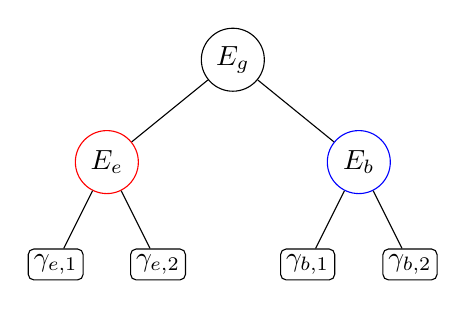
\begin{tikzpicture}[
  grow=down,
  level distance=13mm,
  level 1/.style={sibling distance=32mm},
  level 2/.style={sibling distance=13mm}
]
  \node[state] {$E_g$}
    child foreach \state/\tone in {e/red,b/blue} {
      node[state,draw=\tone] {$E_\state$}
      child foreach \channel in {1,2}
        {node[channel] {$\gamma_{\state,\channel}$}}
    };
\end{tikzpicture}
\end{document}
